\documentclass{beamer-control}
\usepackage{beamer-control-singlefile}
\INCLUDEONLY{Integrator Windup}
\begin{document}
\CONCEPT{Integrator Windup}

\begin{SUMMARY}
\begin{itemize}
\item Saturation and windup
\item Avoiding windup
\end{itemize}
\vfill References:
\begin{itemize}
\item \astrom{§11.4}
\end{itemize}
\end{SUMMARY}



\SUBCONCEPT{Saturation and windup}

\begin{frame}{Actuator saturation}
\begin{itemize}
\item We have mostly analysed control systems from the perspective of linear systems but the effects of nonlinear systems must be considered
\item A nonlinear phenomenon of importance is saturation -- limitations in actuators such as speed limits of motors, region of movement of a robotic arm, or a valves limitations of not being more than fully opened or fully closed
\item All actuators have physical limitations
\end{itemize}
\end{frame}

\begin{frame}{Effect of saturation}
\begin{itemize}
\item When saturation is achieved, the feedback loop is broken and the system effectively runs in open loop with the actuator remaining at the limiting value as long as it is still saturated
\item In these cases, the integral term and the controller input may become very large and it may take a long time for the integrator and controller to come out of saturation
\item This results in very large transient behaviour and is knonwn as \textit{integrator windup}
\item This can occur in any controller with integral action
\end{itemize}
\end{frame}

\begin{frame}{Windup example - cruise control}
\begin{itemize}
	\item Consider the cruise control system when a car encounters a hill (at $t=5$) that is so steep ($6^\circ$) that the throttle saturates when the cruise controller attempts to maintain speed
	\item The torque required is so large that the throttle saturates
\end{itemize}
\begin{figure}
	\centering
	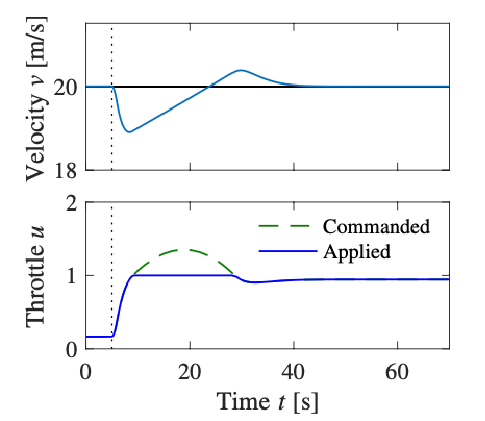
\includegraphics[width=0.5\linewidth]{figure11.10a}
	\\
	\textbf{Figure 11.10 (a)}: Simulation of PI cruise control with windup.
\end{figure}

\end{frame}


\SUBCONCEPT{Avoiding windup}

\begin{frame}{PID controllers}
\begin{itemize}
\item One method for avoiding windup in PID controllers is to add an extra feedback path generated by a model of the saturating actuator
\item We measure the difference between the output of the controller and the actuator model $e_s=u-u_a$ -- when there is no saturation the feedback loop is as normal but at saturation this error signal is fed back to the integrator
\item The result is the controller output is kept close to the saturation limit
\item We can adjust the rate at which the controller output is reset by the gain $k_{aw}$, where a larger gain value indicates a shorter reset time
\end{itemize}
\end{frame}

\begin{frame}{PID controllers}
\begin{figure}
	\centering
	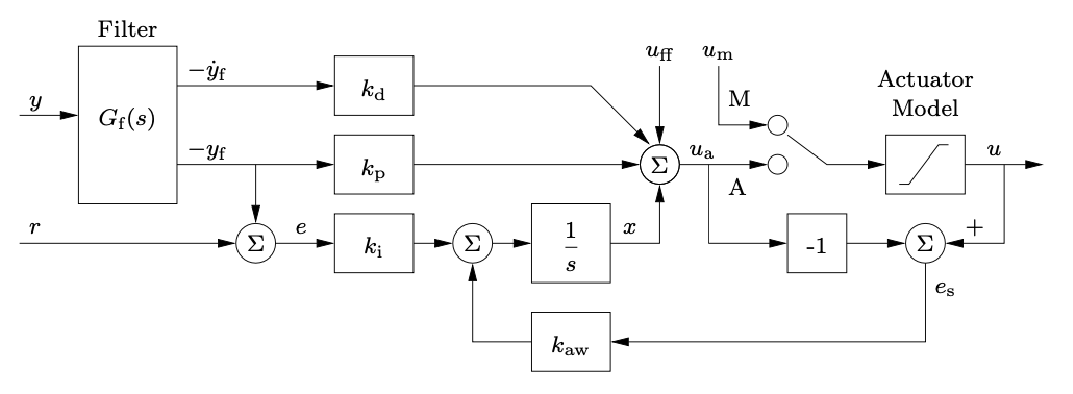
\includegraphics[width=\linewidth]{figure11.11}
	\\
	\textbf{Figure 11.11}: PID controller with filtering, anti-windup, and manual control.
\end{figure}
\end{frame}

\begin{frame}{Anti-windup example - cruise control}
\begin{itemize}
	\item When anti-windup is implemented in the cruise control system, the large overshoot is avoided and the controller output is close to the saturation limit
\end{itemize}
\begin{figure}
	\centering
	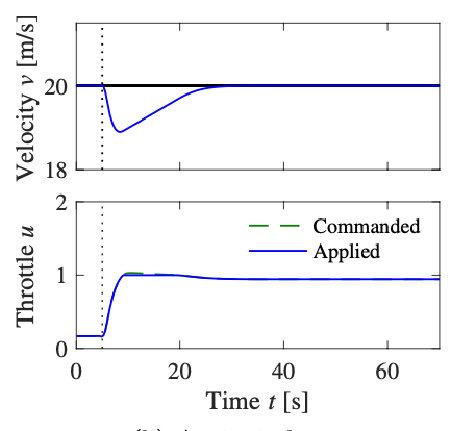
\includegraphics[width=0.5\linewidth]{figure11.10b}
	\\
	\textbf{Figure 11.10 (b)}: Simulation of PI cruise control with anti-windup.
\end{figure}
\end{frame}


\begin{frame}{Manual control and tracking}
	\begin{itemize}
		\item Another method to avoid integral windup is manual control where operation modes are selected by a switch (also seen in Figure 11.11)
		\item The switch is normally set to position A (automatic) and manual control is selected by setting the switch to position M (manual)
		\item In the manual mode of operation, the control variable is manipulated directly by the user
		\item The arrangement shown in Figure 11.11 allows the switching between automatic and manual modes to avoid transients 
	\end{itemize}
\end{frame}


\begin{frame}{Anti-windup for general controllers}
	\begin{itemize}
		\item The ideas for anti-windup for PID controllers can be extended to general controllers like the state space designs seen earlier in the course
		\item We simply need to include a model for the saturating actuator and feed its output back to adjust the entire controller state (instead of just the integrator state)
		\item Below is an example implementing anti-windup to a controller based on state feedback and an observer
\end{itemize}
\begin{figure}
	\centering
	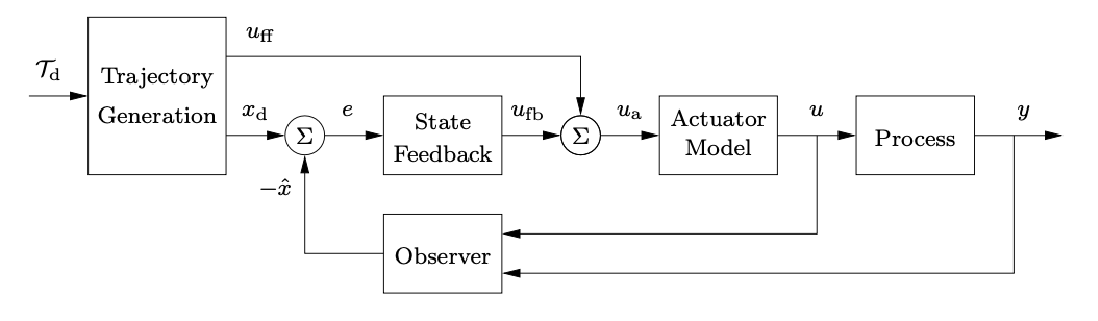
\includegraphics[width=0.9\linewidth]{figure11.12}
	\\
	\textbf{Figure 11.12}: Anti-windup for a general controller architecture.
\end{figure}

\end{frame}


\SUMMARYFRAME
\FINALE

\end{document}
